% По умолчанию используется шрифт 14 размера. Если нужен 12-й шрифт, уберите опцию [14pt]
\documentclass[14pt
  , russian
  %, xcolor={svgnames}
  ]{matmex-diploma-custom}
\usepackage[table]{xcolor}
\usepackage{graphicx}
\usepackage{tabularx}
\newcolumntype{Y}{>{\centering\arraybackslash}X}
\usepackage{amsmath}
\usepackage{amsthm}
\usepackage{amsfonts}
\usepackage{amssymb}
\usepackage{mathtools}
\usepackage{thmtools}
\usepackage{thm-restate}
\usepackage{tikz}
\usepackage{wrapfig}
% \usepackage[kpsewhich,newfloat]{minted}
% \usemintedstyle{vs}
\usepackage[inline]{enumitem}
\usepackage{subcaption}
\usepackage{caption}
\usepackage[nocompress]{cite}
\usepackage{makecell}
%\usepackage{listings}
\usepackage{multicol}
% \setitemize{noitemsep,topsep=0pt,parsep=0pt,partopsep=0pt}
% \setenumerate{noitemsep,topsep=0pt,parsep=0pt,partopsep=0pt}


\graphicspath{ {resources/} }

% 
% % \documentclass 
% %   [ a4paper        % (Predefined, but who knows...)
% %   , draft,         % Show bad things.
% %   , 12pt           % Font size.
% %   , pagesize,      % Writes the paper size at special areas in DVI or
% %                    % PDF file. Recommended for use.
% %   , parskip=half   % Paragraphs: noindent + gap.
% %   , numbers=enddot % Pointed numbers.
% %   , BCOR=5mm       % Binding size correction.
% %   , submission
% %   , copyright
% %   , creativecommons 
% %   ]{eptcs}
% % \providecommand{\event}{ML 2018}  % Name of the event you are submitting to
% % \usepackage{breakurl}             % Not needed if you use pdflatex only.
% 
% \usepackage{underscore}           % Only needed if you use pdflatex.
% 
% \usepackage{booktabs}
% \usepackage{amssymb}
% \usepackage{amsmath}
% \usepackage{mathrsfs}
% \usepackage{mathtools}
% \usepackage{multirow}
% \usepackage{indentfirst}
% \usepackage{verbatim}
% \usepackage{amsmath, amssymb}
% \usepackage{graphicx}
% \usepackage{xcolor}
% \usepackage{url}
% \usepackage{stmaryrd}
% \usepackage{xspace}
% \usepackage{comment}
% \usepackage{wrapfig}
% \usepackage[caption=false]{subfig}
% \usepackage{placeins}
% \usepackage{tabularx}
% \usepackage{ragged2e}
% \usepackage{soul}
\usepackage{csquotes}
% \usepackage{inconsolata}
% 
% \usepackage{polyglossia}   % Babel replacement for XeTeX
%   \setdefaultlanguage[spelling=modern]{russian}
%   \setotherlanguage{english}
% \usepackage{fontspec}    % Provides an automatic and unified interface 
%                          % for loading fonts.
% \usepackage{xunicode}    % Generate Unicode chars from accented glyphs.
% \usepackage{xltxtra}     % "Extras" for LaTeX users of XeTeX.
% \usepackage{xecyr}       % Help with Russian.
% 
% %% Fonts
% \defaultfontfeatures{Mapping=tex-text}
% \setmainfont{CMU Serif}
% \setsansfont{CMU Sans Serif}
% \setmonofont{CMU Typewriter Text}

\usepackage[final]{listings}

\lstdefinelanguage{ocaml}{
keywords={@type, function, fun, let, in, match, with, when, class, type,
nonrec, object, method, of, rec, repeat, until, while, not, do, done, as, val, inherit, and,
new, module, sig, deriving, datatype, struct, if, then, else, open, private, virtual, include, success, failure,
lazy, assert, true, false, end},
sensitive=true,
commentstyle=\small\itshape\ttfamily,
keywordstyle=\ttfamily\bfseries, %\underbar,
identifierstyle=\ttfamily,
basewidth={0.5em,0.5em},
columns=fixed,
fontadjust=true,
literate={->}{{$\to$}}3 {===}{{$\equiv$}}1 {=/=}{{$\not\equiv$}}1 {|>}{{$\triangleright$}}3 {\\/}{{$\vee$}}2 {/\\}{{$\wedge$}}2 {>=}{{$\ge$}}1 {<=}{{$\le$}} 1,
morecomment=[s]{(*}{*)}
}

\lstset{
mathescape=true,
%basicstyle=\small,
identifierstyle=\ttfamily,
keywordstyle=\bfseries,
commentstyle=\scriptsize\rmfamily,
basewidth={0.5em,0.5em},
fontadjust=true,
language=ocaml
}
 
\newcommand{\cd}[1]{\texttt{#1}}
\newcommand{\inbr}[1]{\left<#1\right>}


\newcolumntype{L}[1]{>{\raggedright\let\newline\\\arraybackslash\hspace{0pt}}m{#1}}
\newcolumntype{C}[1]{>{\centering\let\newline\\\arraybackslash\hspace{0pt}}m{#1}}
\newcolumntype{R}[1]{>{\raggedleft\let\newline\\\arraybackslash\hspace{0pt}}m{#1}}



\usepackage{soul}
\usepackage[normalem]{ulem}
%\sout{Hello World}

\usepackage{newfloat,caption,float}
\usepackage{newfloat}
\usepackage{subcaption}

\DeclareFloatingEnvironment[
	fileext = loe,
	listname = Examples, 
	name = Листинг,
	placement = H,
	within = none,
]{example}
\captionsetup[example]{labelfont=bf}

%\newcommand\theexample{\alph{subexample}}
%\newcommand\thesubexample{\alph{subexample}}
% \newcommand\p@subexample{\theexample}

%\DeclareCaptionSubType{#1} 
%\renewcommand\thesubexample{\theexample\alph{subexample}}
\ForEachFloatingEnvironment{\DeclareCaptionSubType*{#1}}
\captionsetup[subexample]{labelformat=simple}

\newcommand{\ReasonML}{\textsc{ReasonML}}
\newcommand{\OCaml}{\textsc{OCaml}}
\newcommand{\ocamllex}{\textsc{ocamllex}}
\newcommand{\ocamlyacc}{\textsc{ocamlyacc}}
\newcommand{\merlin}{\textsc{merlin}}

\ifx\pdfoutput\undefined
\usepackage{graphicx}
\else
\usepackage[pdftex]{graphicx}
\fi
\usepackage{float}
\usepackage{caption}
\usepackage{subcaption}


\begin{document}
\input{title.tex}
\maketitle
\setcounter{tocdepth}{2}
\tableofcontents

\section{Введение}
Reason~--- это расширение синтаксиса OCaml и новый набор инструментов, созданные в Facebook в 2016 году. Для языка был придуман C-подобный синтаксис, так же похожий и на JavaScript, что бы программистам, пишущим на этих языках, было легче адаптироваться\cite{RE}. Одной из целей создания нового языка было упрощение взаимодействия с JavaScript, добавление поддержки JSX и возможности компиляции в JavaScript\cite{WE}. В наследство от OCaml Reason-у досталась возможность компилироваться в нативный и переносимый коды, а так же система типов со всеми преимуществами, такими как уменьшение количества ошибок в программах и повышение удобства поддержки кода.

Однако существует проблема у людей, уже пишущих на OCaml. Так как Reason остался достаточно похожим на него, в языках имеются одинаковые синтаксические конструкции, отличающиеся только оформлением. Из-за этого довольно сложно переключиться на новый синтаксис, и, как следствие, программист по ошибке может написать вполне корректный для OCaml участок кода, но не подходящий для Reason. В таком случае стоит указать человеку на его ошибку предупреждением и продолжить синтаксический анализ программы, корректно прочитав конструкцию из чужого языка.

Таким образом, актуальной задачей является добавление новых правил в синтаксический анализатор Reason с восстановлением от типичных ошибок, вызванных смешением языков.

\section{Постановка задачи}
\label{sec:task}
% !TeX spellcheck = ru_RU
Целью данной работы является дополнение существующего парсера Reason новыми правилами восстановления от ошибок, вызванных смешением синтаксиса Reason и OCaml.

Для её выполнения были поставлены следующие задачи:
 \begin{enumerate}
 \item Исследовать предметную область:
 \begin{enumerate} 
 	\item Рассмотреть принципы работы LR(1) анализаторов.
	\item Рассмотреть принцип работы генераторов синтаксических анализаторов.
 	\item Изучить существующую реализацию синтаксического анализатора на OCaml (Menhir).
 \end{enumerate}
 \item Реализовать дополнительные правила восстановления от ошибок.
 \item Реализовать в merlin и Reason предупреждения о смешении кода разных языков.
 \item Реализовать в ocaml-lsp автоматическое исправление кода OCaml, добавленного в Reason.
 \item Реализовать в ocaml-lsp автоматическое исправление кода Reason, добавленного в OCaml.
 
 \end{enumerate}

\section{Обзор}
\label{sec:relatedworks}

\subsection{Синтаксические анализаторы}
Синтаксический анализ или парсинг (parsing)~--- процесс сопоставления последовательности токенов (лексем) дерева разбора, называемого абстрактным синтаксическим деревом (AST).

Синтаксический анализатор или парсер (parser)~--- это программа, выполняющая синтаксический анализ.

Так же от синтаксического анализатора ожидаются сообщения обо всех выявленных ошибках, причем достаточно внятные и полные, а кроме того, умение обрабатывать обычные, часто встречающиеся ошибки и продолжать работу с оставшейся частью программы.
Имеется три основных типа синтаксических анализаторов: универсальные, восходящие и нисходящие\cite{DB}. Мы остановимся на восходящем анализе. Восходящие синтаксические анализаторы строят дерево разбора начиная с листьев (снизу) и идя к корню (вверх). Поток символов сканируется последовательно --- слева направо.

Здесь будет рассмотрен общий вид восходящего анализа типа <<перенос/свёртка>> (shift-reduce). При анализе типа перенос-свёртка для хранения символов грамматики используется стек, а для хранения остающейся непроанализированной части входной строки~--- входной буфер. На каждом шаге свёртки (reduction) определенная подстрока, соответствующая правой части продукции, заменяется на нетерминал, являющийся левой частью продукции. Основа~--- это подстрока, которая соответствует телу продукции и свертка которой представляет собой один шаг правого порождения в обратном порядке. Использование стека в анализаторе объясняется тем важным фактом, что {\it основа} всегда находится на вершине стека и никогда~--- внутри него.

LR(k)-грамматики~--- это грамматики, для которых может быть построен синтаксический анализатор, работающий по принципу переноса-свёртки.

Наиболее эффективные восходящие методы работают только с подклассами грамматик, однако некоторые из этих классов, такие как LR(k) грамматики, достаточно выразительны для описания большинства синтаксических конструкций языков программирования.
L~--- здесь означает сканирование входного потока слева направо, R~--- построение правого порождения в обратном порядке, а k --- количество предпросматриваемых символов входного потока, необходимых для принятия решения. 

Одними из самых эффективных синтаксических анализаторов являются LR(1)\cite{LRSpeed}. LR(1)-анализатор состоит из входного буфера, выхода, стека, программы-драйвера и таблицы синтаксического анализа. Программа-драйвер одинакова для всех LR-анализаторов, от одного анализатора к другому меняются таблицы синтаксического анализа. Программа ситаксического анализатора по одному считывает символы из входного буфера. После прочтения очередного символа она обращается к управляющей таблице и совершает соответствующее действие. Процесс чтения продолжается, пока входная цепочка не закончится.

\subsection{Menhir}
Построение анализаторов LR(1) вручную достаточно трудоемкий процесс, поэтому чаще всего пользуются генераторами синтаксических анализаторов. 

Генератор синтаксических анализаторов --- это программа, которая по спецификации грамматики строит синтаксический анализатор. Одним из таких генераторов и является Menhir~\cite{ME}. Он был выбран командой Reason, как лучшая, по сравнению с ocamlyacc~\cite{ocamlyacc}, версия генераторов синтаксических анализаторов.



\subsection{Примеры ошибок}

Здесь будут приведены примеры синтаксических конструкций, в которых часто встречаются ошибки, в формате сравнения кода на OCaml и Reason соответственно.

\hfill


\begin{example}
	\begin{subexample}[b]{\textwidth}
		\lstinputlisting[frame=single,language=Caml]{examplePatternMatching.ml}
		\caption{Код OCaml}
	\end{subexample}
	\hfill
	
	\begin{subexample}[b]{\textwidth}
		\lstinputlisting[frame=single, language=Caml]{examplePatternMatching.re}
		\caption{Код Reason}
	\end{subexample}
\caption{Сопоставление с образцом}\label{l1}
\end{example}

На листинге \ref{l1} представлена конструкция сопоставления с образцом (pattern matching). Программист может перепутать оформление стрелок (-> и =>), выбрать ключевые слова из другого языка ({\it match - with} и {\it switch(-)}) или забыть поставить фигурные скобки.


\hfill


\begin{example}
%\begin{multicols}{2}
	\begin{subexample}{0.5\textwidth}
		\lstinputlisting[frame=single, language=Caml]{forloop.ml}
		\caption{Код OCaml}
	\end{subexample}
	\begin{subexample}{0.5\textwidth}
		\lstinputlisting[frame=single, language=Caml]{forloop.re}
		\caption{Код Reason}
	\end{subexample}
%\end{multicols}
\caption{Пример цикла}\label{l2}
\end{example}

На листинге \ref{l2} представлен стандартный цикл. Человек может вместо фигурных скобок заключать тело цикла в {\it do} и {\it done}, неправильно инициализировать переменную ({\it i = 1} и {\it i in 1}) или забыть фигурные скобки после {\it for}.


\hfill


\begin{example}
%\begin{multicols}{2}
	\begin{subexample}{0.5\textwidth}
		\lstinputlisting[frame=single, language=Caml]{record.ml}
		\caption{Код OCaml}
	\end{subexample}
	\begin{subexample}{0.5\textwidth}
		\lstinputlisting[frame=single, language=Caml]{record.re}
		\caption{Код Reason}
	\end{subexample}
%\end{multicols}
\caption{Пример записи}\label{l3}
\end{example}

На листинге \ref{l3} приведено описание типа, называемого записью. В первом случае поля отделяются точкой с запятой, во втором случае просто запятой.

\subsection{Merlin}

Проект \merlin{}\cite{mer} является реализацией сервера для анализа языка \OCaml{} (language server). Чаще всего он подключается к редакторам текста с помощью различных расширений этих редакторов, чтобы разработчик мог использовать редактор как современную интегрированную среду разработки (IDE), т.\,е. пользоваться переходом к определению объявленных имен, автодополнением и т.\,п. На данный момент в исходном коде \ReasonML{} имеется расширение для \merlin{}, которое позволяет использовать \merlin{} не только для редактирования кода на \OCaml{}, но и на \ReasonML{}.

В контексте данной работы выглядит интересной задача тесной интеграции синтаксического анализатора с проектом \merlin{}, а именно добавление возможности быстрого исправления кода, написанного со смешением двух языков, на правильный код на \ReasonML{}.


%\subsection{Реализация дополнительных правил}



\section{Результаты}
\subsection{Reason}
В Reason добавлены следующие возможности:
\begin{itemize}

\item Можно использовать другой стиль стрелок («->» вместо «=>») в pattern matching.%, но в таком случае не работает {\it when} (одна из дополнительных функций).

\item Можно писать pattern matching в стиле \OCaml{}.%, но тогда после стрелки может идти только единичное выражение, а не их последовательность.%\footnote[1]{Однако эта проблема легко решается заключением последовательности в \{\}. }

\item Можно писать условие и тело цикла в стиле \OCaml{}.

\item Можно использовать разделитель <<;>> вместо <<,>> в объявлении record.

\item Можно объявлять модули в стиле \OCaml{}.

\item Можно писать {\it if} с {\it then}.

\item Добавлено ключевое слово {\it match}.% и теперь оно не может использоваться в качестве идентификатора.

\end{itemize}

Так же добавлены предупреждения (warning) для всех синтаксических конструкций перечисленных выше. И реализовано быстрое исправление кода (<<Quick fix>>) в OCaml-LSP, которое заменяет {\it match with} и {\it struct end} на подходящие языку Reason ключевые слова.
\begin{figure}[h]
%\fbox{
	\begin{subfigure}[t]{0.5\textwidth}
		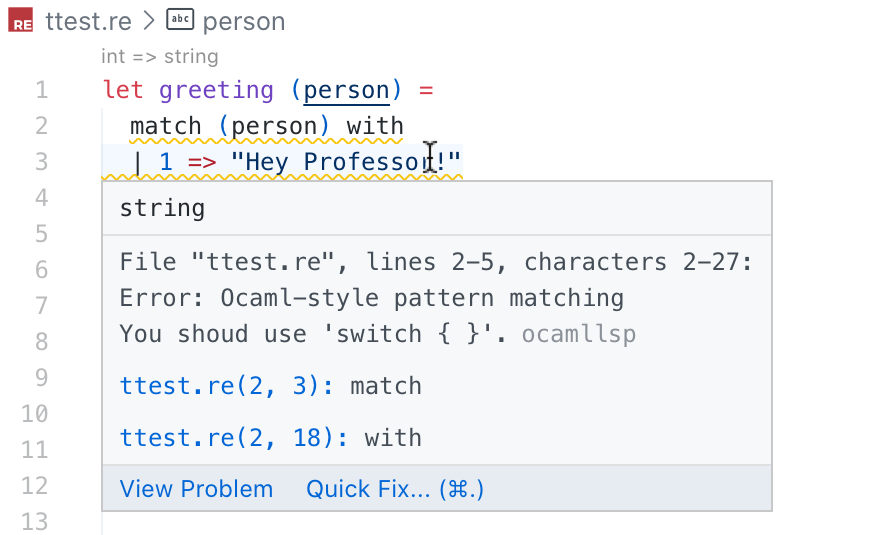
\includegraphics[width=\linewidth]{screenshots/05.png}
		\caption{IDE предупреждает о том, что pattern matching написан в стиле OCaml и \newline предлагает быстрое исправление.}
	\end{subfigure}
%}
	\begin{subfigure}[t]{0.5\textwidth}
		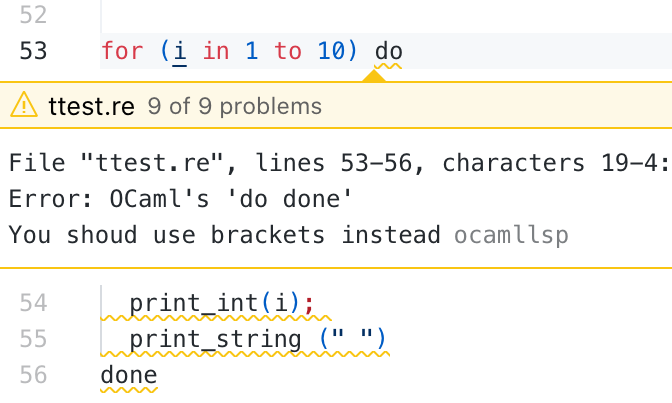
\includegraphics[width=\linewidth]{screenshots/06.png}
		\caption{IDE предупреждает о том, что цикл написан в стиле OCaml.}
	\end{subfigure}
\caption{Примеры предупреждений в коде Reason}
\end{figure}
\newpage
\subsection{OCaml}
Для симметричной задачи, для OCaml реализованы предупреждения в OCaml-LSP для следующих конструкций из Reason: определение модуля, pattern matching (при этом стрелки должны быть из OCaml), запятые в record. Для этих же конструкций реализованы соответствующие быстрые исправления в OCaml-LSP:
\begin{itemize}

\item Замена {\it \{ \}} на {\it struct end}.

\item Замена {\it switch \{ \}} на {\it match with}.

\item Замена всех <<,>> на <<;>> в объявлении record.

\end{itemize}

\begin{figure}[h]
	\begin{subfigure}[t]{0.5\textwidth}
		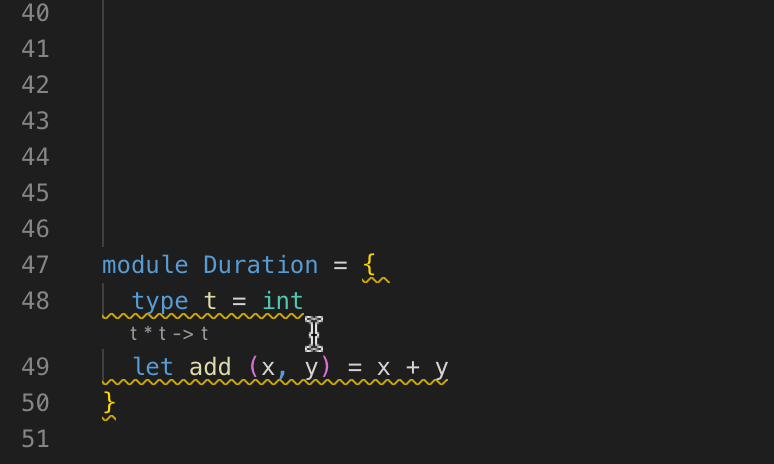
\includegraphics[width=\linewidth]{screenshots/01.png}
		\caption{Неверно написанная конструкция выделяется цветной волной.}
	\end{subfigure}
	\begin{subfigure}[t]{0.5\textwidth}
		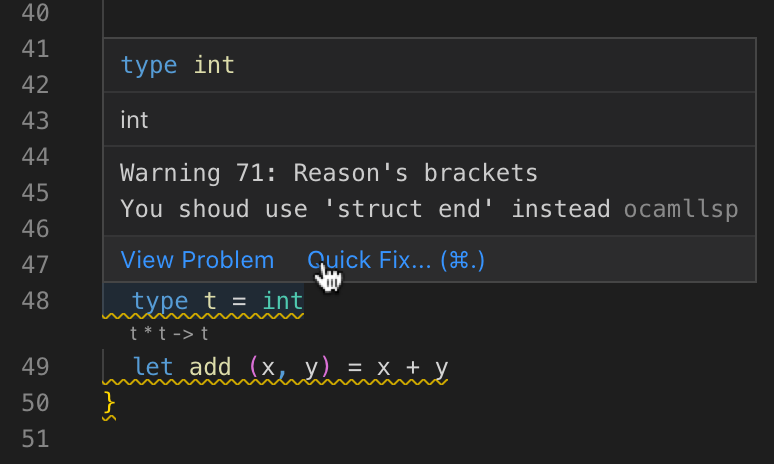
\includegraphics[width=\linewidth]{screenshots/02.png}
		\caption{IDE предлагает <<Quick fix>>.}
	\end{subfigure}
	\newline
	\begin{subfigure}{0.5\textwidth}
		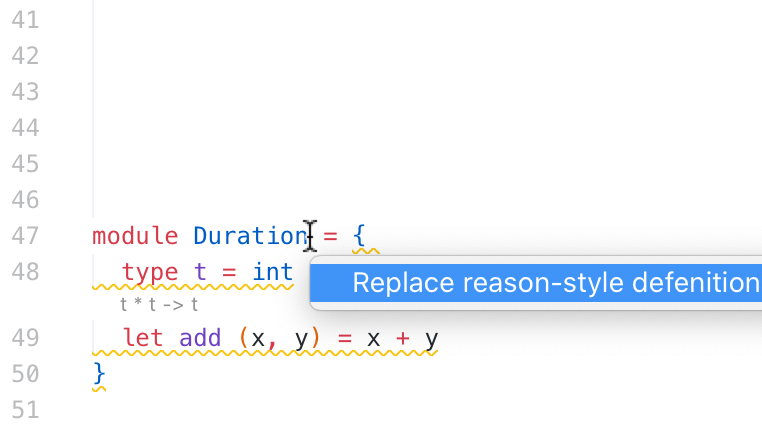
\includegraphics[width=\linewidth]{screenshots/03.png}
		\caption{Кнопка запускающая замену.}
	\end{subfigure}
	\begin{subfigure}{0.5\textwidth}
		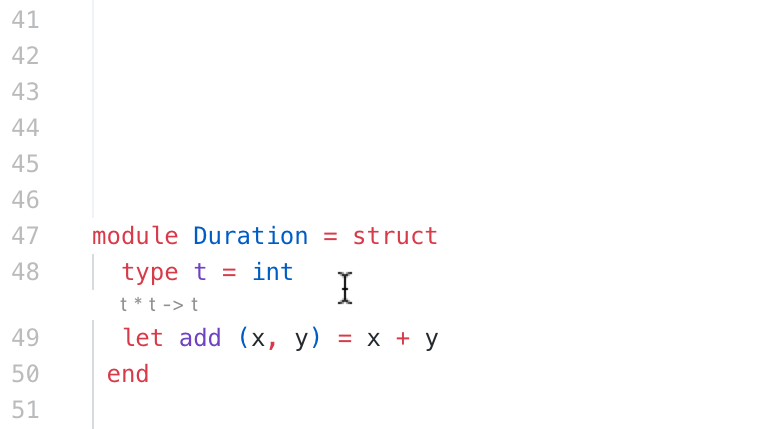
\includegraphics[width=\linewidth]{screenshots/04.png}
		\caption{Исправленная конструкция.}
	\end{subfigure}
\caption{Исправление кода OCaml}
\end{figure}

\newpage

\subsection{Архитектура}
\begin{figure}[h]
	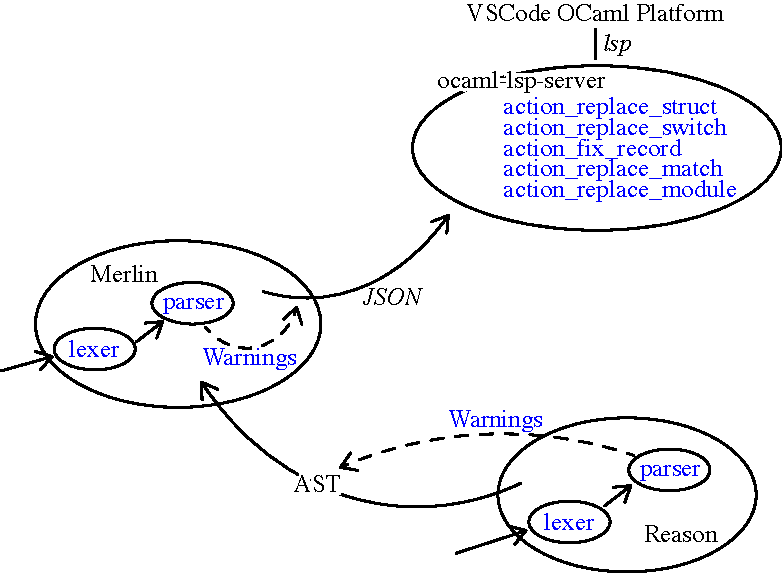
\includegraphics[width=\linewidth]{graph.pdf}
\caption{Архитектура расширения. Стрелки обозначают передачу данных. Курсивом выделены протоколы. Синим цветом выделены части, которые подверглись изменениям, зеленым~--- новые модули.}
\end{figure}
Поддержка OCaml в Reason реализована через новые синтаксические правила для парсера. Для этих правил так же созданы предупреждения (warnings), как новый тип reason\_warning, по примеру существующего в Reason типа reason\_error. Во время работы парсера предупреждения выкидываются из него и собираются. Далее они, с помощью добавленной функции warning\_attribute, превращаются в атрибуты AST и вместе с ним передаются в merlin, откуда идут в ocaml-lsp и в итоге в IDE. Необходимая поддержка атрибутов reason.warning добавлена на стороне merlin.

Поддержка Reason в OCaml реализована через новые правила для парсера и расширение стандартного списка предупреждений OCaml.

Стоит заметить, что для Reason реализована поддержка второго языка как при {\it компиляции}, так и в {\it IDE}, тогда как у OCaml только для {\it IDE}. Такая ситуация возникла из-за того, что у Reason одна кодовая база для парсера, компилятора и reason-merlin, в отличии от OCaml, где два разных репозитория для компилятора и Merlin. В нашем случае частичная поддержка Reason была добавлена только в Merlin.

Функции исправления кода в ocaml-lsp как для Reason, так и для OCaml созданы по примеру action\_add\_rec\footnote{ \url{https://github.com/ocaml/ocaml-lsp/blob/1.13.1/ocaml-lsp-server/src/code_actions/action_add_rec.ml} (дата доступа: 24.08.2022) }. Action\_add\_rec~--- это code\-Action, добавляющий слово {\it rec} перед рекурсивной функцией, если его еще не было. CodeAction, являющийся частью спецификации протокола lsp, представляет собой изменение, которое может быть выполнено в коде, например для рефакторинга кода.

\subsection{Установка}
Необходимая для ocaml-lsp версия OCaml~--- 4.13.1/4.13. Reason совместим с версиями 4.13.1/4.13/4.12.1/4.12. Так же понадобится opam. Все необходимые пакеты устанавиваются следующими командами:

% ":" not italic, i don't know
\lstset{emph={https}, emphstyle={\itshape \small} }
\lstset{basicstyle=\ttfamily}
\begin{example}
\begin{lstlisting}[frame=single,
language=C,
% fix stupid bug with bad "-" in copying from pdf
literate={-}{-}1
]
opam pin add reason https://github.com/pereb4ik/reason.git
opam pin add ocaml-lsp-server https://github.com/pereb4ik/ocaml-lsp.git
\end{lstlisting}
\caption{Команды установки Reason и ocaml-lsp}
\end{example}
Для тестирования функций IDE таких, как умная замена кода <<Quick fix>>, понадобится Visual Studio Code (хотя ocaml-lsp можно использовать с другими редакторами) с расширением OCaml Platform от OCaml Labs.

Результаты проделанной работы можно наблюдать в соответсвующих репозиториях. Ссылки на списки коммитов Reason\footnote{ \url{https://github.com/pereb4ik/reason/commits?author=pereb4ik} (дата доступа: 8.08.2022) },
OCaml-LSP\footnote{ \url{https://github.com/pereb4ik/ocaml-lsp/commits?author=pereb4ik} (дата доступа: 8.08.2022) },
merlin\footnote{ \url{https://github.com/pereb4ik/merlin/commits/lsp?author=pereb4ik} (дата доступа: 8.08.2022) }.

\section{Заключение}
В рамках данной работы было проведено подготовительное исследование возможности расширения синтаксического анализатора \ReasonML{} правилами для языка \OCaml{}. В ходе исследования были выполнены и начата работа над следующими задачами.


\begin{enumerate}
\item[\checkmark] Исследовать предметную область:
\begin{enumerate} 
\item[\checkmark] Рассмотреть принципы работы LR(1) анализаторов.
\item[\checkmark] Рассмотреть принцип работы генераторов синтаксических анализаторов.
\item[\checkmark] Изучить существующую реализацию синтаксического анализатора на \OCaml{} (Menhir).
\end{enumerate}
\item[\checkmark] Реализовать дополнительные правила восстановления от ошибок.
\item[$\times$] Оценить качество восстановления от ошибок.
\end{enumerate}

\noindent В процессе работы возникали опасения того, что лексический анализатор \ReasonML{} на основе \ocamllex{} потребует доработки. Однако, большинство полезных лексем там уже поддерживается и добавление новых не должно вызвать серьёзных усилий. 

В оставшийся срок работы планируется реализовать изменения в синтаксическом анализаторе \ReasonML{} для улучшения поддержки синтаксических конструкций языка \OCaml{}. При удачном стечении обстоятельств планируется доработать \merlin{} и расширение для редактора \textsc{VsCode} поддержкой возможностей автоматического исправления кода, написанного с использованием смешения языков.

В планах на будущее выглядит интересным не только улучшение синтаксического анализатора \ReasonML{} для облегчения жизни программистам на \OCaml{}, но и наоборот: доработка синтаксического анализатора \OCaml{} в проекте \merlin{} для более удобной миграции программистов на \ReasonML{} в сообщество языка \OCaml{}.


% \nocite{*}
\setmonofont[Mapping=tex-text]{CMU Typewriter Text}
\bibliographystyle{ugost2008ls}
\bibliography{vkr}
\end{document}
